\section{Позиционные пневмоприводы с дискретными распределителями}

Проведенный анализ развития позиционных пневмоприводов показывает, что многие существующие 
решения основаны на применении пропорциональной техники,
обеспечивающей плавное регулирование расхода воздуха. Однако в современных условиях особую актуальность приобретает
задача создания систем на базе дискретных распределителей, что обусловлено их существенно меньшей
стоимостью, более высокой надежностью и лучшей совместимостью с цифровыми системами управления.

Характерной особенностью позиционных пневмоприводов с дискретными распределителями является то, что они могут рассматриваться как системы с переменной
структурой. В процессе работы такие системы претерпевают качественные изменения своей структуры, обусловленные переключением распределителей, что приводит к
существенному изменению динамических свойств привода на различных этапах движения.

Проведенный анализ современного состояния исследований выявил существенные пробелы в текущем понимании проблемы функционирования
таких систем. В первую очередь отсутствует комплексный подход к оценке эффективности различных структур позиционных пневмоприводов с дискретными распределителями.
Существующие публикации, как правило, фокусируются на отдельных показателях качества, таких как точность или быстродействие, без учета их взаимного влияния. При этом
недостаточно исследована проблема взаимосвязи между повышением точности позиционирования и увеличением частоты переключений распределителей, что напрямую влияет на износ оборудования и его ресурс.

Анализ особенностей функционирования этих систем выявляет три противоречивых требования: обеспечение высокой точности
позиционирования, достижение требуемого быстродействия и минимизация количества переключений распределителей. Повышение точности
требует более частого переключения распределителей для коррекции положения штока, что приводит к ускоренному износу распределительной аппаратуры и снижению ресурса системы.
В свою очередь, увеличение быстродействия может негативно сказаться на точности из-за возрастания динамических ошибок, а стремление к минимизации числа переключений ограничивает
возможности как точной коррекции положения, так и обеспечения требуемого быстродействия.

Существующие методики многокритериальной оптимизации параметров таких систем не обеспечивают требуемой эффективности.
Для решения данной задачи целесообразно применение аппарата Парето-оптимизации, позволяющего построить множество недоминируемых решений в
пространстве трех критериев. Построение фронта Парето дает возможность выявить предельно достижимые характеристики системы при различных соотношениях
критериев, научно обосновать выбор рациональных параметров с учетом конкретных требований к точности, быстродействию и ресурсу, а также оценить
эффективность различных структур пневмоприводов с позиции многокритериальной оптимальности.

Управление подобными системами требует особого подхода, учитывающего наличие ограниченного числа возможных состояний, определяемых комбинациями положений
дискретных распределителей. При этом существенная нелинейность динамических процессов, обусловленная как физическими свойствами сжатого воздуха,
так и дискретным характером управляющих воздействий, создает дополнительные сложности при разработке алгоритмов управления.

Для эффективного решения задачи позиционирования принципиально важным является интегративный подход к проектированию таких систем. Попытки оптимизации отдельных подсистем
без учета их взаимного влияния, как показывает практика, не позволяют достичь требуемых показателей качества. Это обусловлено тесной взаимосвязанностью процессов в
пневматической, механической и управляющей подсистемах. Термодинамические процессы в полостях пневмоцилиндра определяют динамику механической части, которая в свою
очередь влияет на алгоритмы переключения распределителей, что в конечном итоге отражается на позиционировании. Такая взаимосвязь исключает возможность независимого
рассмотрения подсистем и требует комплексного подхода к проектированию.

Развитие данного направления можно проследить через ряд исследовательских работ и патентных решений, предлагающих различные подходы к реализации дискретного управления пневмоприводами.

Так, в работе И.Б. Филиппова \cite*{филиппов:позиц_след_пневмопривод} рассматриваются особенности позиционных пневматических механизмов
с дискретным управлением, предназначенных для перемещения выходных звеньев или объектов из точки в точку по
заданной программе. Отмечается, что для таких механизмов основными требованиями являются обеспечение максимального
быстродействия и необходимой точности позиционирования при ограниченных динамических нагрузках.

Описывается конструкция и принцип работы разработанного позиционного пневмопривода с одной дискретно управляемой полостью, представленного
на рисунке \cref*{fig:позиционный_пп_филипов}.

\begin{figure}[h]
	\centerfloat
	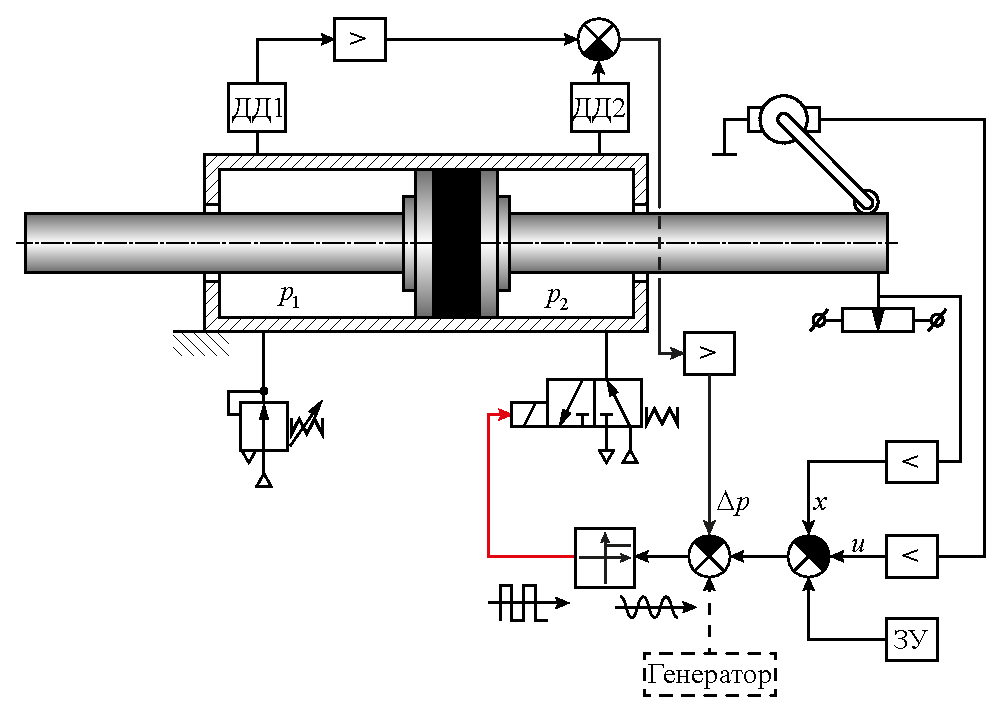
\includegraphics{philipov_positinon_act.eps}
	\caption{Схема дискретного пневмопозиционера}\label{fig:позиционный_пп_филипов}
\end{figure}

Его силовая часть состоит из пневмоцилиндра, в поршневой полости которого редукционным клапаном поддерживается
постоянное давление, а в штоковой полости давление регулируется трехлинейным двухпозиционным распределителем. Измерительная
часть включает датчики давления, тахогенератор и потенциометр для обратных связей по перемещению, скорости и перепаду
давления. Управление движением сводится к управлению торможением и позиционированием за счет переключения распределителя,
соединяющего штоковую полость то с магистралью, то с атмосферой.

Автор отмечает, что вследствие колебания давления в штоковой полости уменьшается влияние зоны нечувствительности,
определяемой сухим трением. Приведены результаты исследований, показывающие, что частота переключения распределителя определяется
его собственным временем запаздывания и мало зависит от других параметров, что позволяет избежать автоколебаний даже
в наиболее неблагоприятных точках позиционирования.

Дополнительные возможности открывает применение вибрационного сглаживания нелинейностей вынужденными колебаниями.
В этом случае при достижении сигналом рассогласования величины амплитуды гармонического воздействия клапан переходит
в режим постоянного переключения, поддерживая давление в управляемой полости таким, чтобы обеспечить торможение и точное
позиционирование. Преимуществом данного алгоритма является возможность задавать частоту вынужденных колебаний для
обеспечения необходимого качества переходного процесса и требуемого запаса устойчивости.

Дальнейшим шагом стало комплексное рассмотрение Г.А. Крутиковым, А.И. Кудрявцевым и Л.А. Пекарем \cite*{крутиков:способы_торможения_12}
способов торможения поршня пневмопривода без использования специальных тормозных устройств. В работе
рассмотрено 12 схем торможения пневмопривода, разделенные на 3 основные группы (I, II, III), показанные на рисунке \cref*{fig:эффективные_схемы_торможения_12}.

\begin{figure}[h]
    \centerfloat
    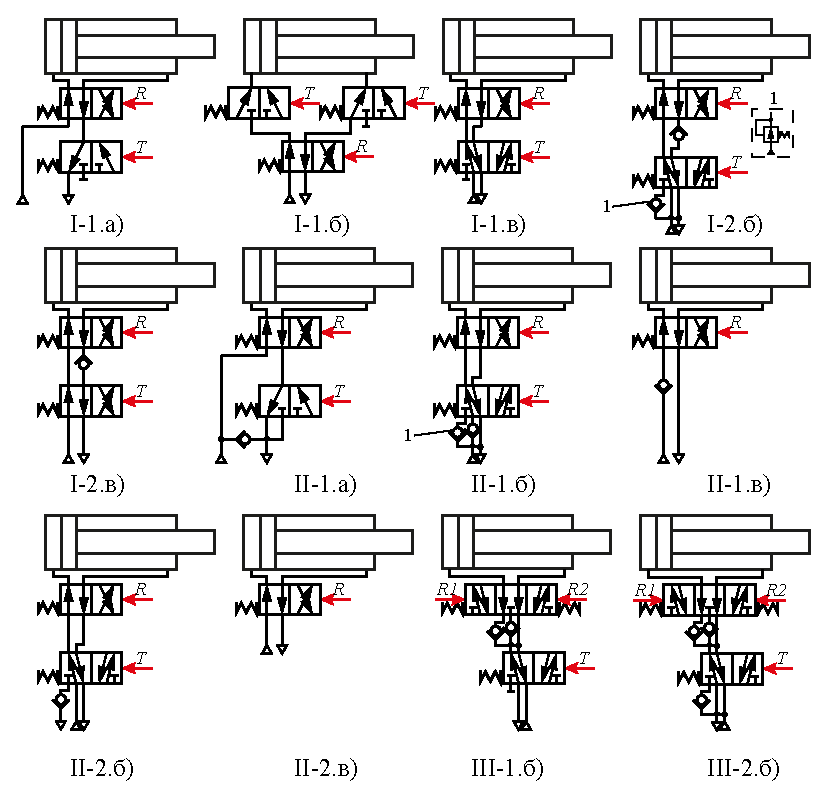
\includegraphics{kurtikob.eps}
    \caption{Эффективные схемы торможения пневмопривода}\label{fig:эффективные_схемы_торможения_12}
\end{figure}

Отличительной особенностью этих схем является отсутствие регулируемых дросселей и емкостей ---
настройка оптимального режима торможения осуществляется только изменением тормозного пути.

Оценка эффективности каждой схемы осуществлялась по ряду ключевых критериев: время срабатывания пневмопривода,
относительная масса сжатого воздуха, потребляемого за один цикл, осредненный за цикл КПД пневмопривода, максимальное
ускорение при торможении, максимальная степень сжатия воздуха в тормозной полости, относительная стоимость
аппаратурной реализации и относительный тормозной путь. Для объективного сравнения каждой схеме была дана оценка в
баллах от 1 до 10 по каждому из показателей, причем максимальный балл присваивался схеме с наилучшим значением
параметра. Коэффициенты значимости различных критериев были определены экспертным методом в соответствии с
рекомендациями.

Наилучшие комплексные показатели качества продемонстрировали схемы III-2.б и III-1.б, которые, несмотря на
более высокую стоимость реализации, обладают лучшими энергетическими характеристиками, высоким быстродействием
и более плавным режимом торможения. Принципиальное отличие этих схем группы III заключается в том, что в них
используется не только вторая составляющая удельной работы сжатого воздуха (изотермическое расширение), но и его
потенциальная энергия, что существенно повышает КПД пневмопривода.

Особого внимания заслуживает схема I-2.б с обратным клапаном, которая позволяет устранить недостатки схемы I-1.б
с высокими пиковыми ускорениями и отскоком поршня. Максимальное ускорение в этом случае снижается с 15,5~\si{\metre\per\square\second}
до 4,16~\si{\metre\per\square\second}, отскок минимален, а время срабатывания составляет 1,05~\si{\second}. Энергетические характеристики также улучшаются
за счет частичной рекуперации воздуха из тормозной полости.

Дальнейшее улучшение режима торможения обеспечивает модификация схемы I-2.б с установкой редукционного клапана вместо
обратного. Это позволяет реализовать практически равнозамедленный режим торможения с постоянным отрицательным
ускорением 1,38~\si{\metre\per\square\second}, полностью устраняет отскок поршня и обеспечивает предохранение тормозной полости от недопустимо
высоких давлений. Основными преимуществами такой схемы являются мягкий и плавный режим торможения с регулируемым
ускорением, экономное использование сжатого воздуха за счет рекуперации, высокое быстродействие и удобство настройки.

Таким образом, комплексная оценка и сравнение различных схем торможения пневмопривода, проведенная авторами, позволила
выявить наиболее эффективные решения. В частности, схема I-2.б с редукционным клапаном демонстрирует оптимальное
сочетание высокого быстродействия, плавного режима торможения с заданным ускорением, экономного расхода сжатого
воздуха и защиты тормозной полости от чрезмерных давлений. Эта схема рекомендуется авторами для использования в качестве
внешнего тормозного устройства для пневмопривода с большими инерционными нагрузками.

В настоящее время, благодаря стремительному развитию микроэлектроники и её применению в различных
областях, стало возможным использование сложных алгоритмов управления. Эти достижения позволяют решать
многие отмеченные ранее вопросы с помощью более гибких систем управления.

Однако применение алгоритмов, предназначенных для непрерывных систем, к системам с
дискретными элементами может быть затруднительным или даже невозможным. Часто при использовании
ПИД-регулятора исследователи применяют различные преобразователи и модуляции сигнала. Например,
широко распространено использование широтно-импульсной модуляции (ШИМ) в сочетании с ПИД.
